%TODO: check that we only use 'systems' (isntead of method, algorithm, comp model) and 'metrics' (instead of measures)
% -----------------------------------------------
% Template for ISMIR Papers
% 2016 version, based on previous ISMIR templates

% Requirements :
% * 6+1 page length maximum
% * 2MB maximum file size
% * Copyright note must appear in the bottom left corner of first page
% (see conference website for additional details)
% -----------------------------------------------

\documentclass{article}
\usepackage{ismir,amsmath,cite}
\usepackage{url}
\usepackage{cleveref}
\usepackage{graphicx}
\usepackage{color}
% \usepackage{hyperref}
\graphicspath{{figs/}}
\usepackage{booktabs}
\usepackage{enumitem}

\setlist[itemize]{noitemsep, topsep=0ex}
\setlist[enumerate]{noitemsep, topsep=0ex}

\def\eg{\emph{e.g.\/}}
\def\ie{\emph{i.e.\/}}
\def\etc{\emph{etc.\/}}
\def\etal{\emph{et al.\/}}


% Title.
% ------
\title{A Plan for Sustainable MIR Evaluation}

% Note: Please do NOT use \thanks or a \footnote in any of the author markup

% Single address
% To use with only one author or several with the same address
% ---------------
%\oneauthor
% {Names should be omitted for double-blind reviewing}
% {Affiliations should be omitted for double-blind reviewing}

% Two addresses
% --------------
%\twoauthors
%  {First author} {School \\ Department}
%  {Second author} {Company \\ Address}

%% To make customize author list in Creative Common license, uncomment and customize the next line
%  \def\authorname{First Author, Second Author}


% Three addresses
% --------------
\threeauthors%
  {First Author} {Affiliation1 \\ {\tt author1@ismir.edu}}
  {Second Author} {\bf Retain these fake authors in\\\bf submission to preserve the formatting}
  {Third Author} {Affiliation3 \\ {\tt author3@ismir.edu}}

%% To make customize author list in Creative Common license, uncomment and customize the next line
%  \def\authorname{First Author, Second Author, Third Author}

% Four or more addresses
% OR alternative format for large number of co-authors
% ------------
%\multauthor
%{First author$^1$ \hspace{1cm} Second author$^1$ \hspace{1cm} Third author$^2$} { \bfseries{Fourth author$^3$ \hspace{1cm} Fifth author$^2$ \hspace{1cm} Sixth author$^1$}\\
%  $^1$ Department of Computer Science, University , Country\\
%$^2$ International Laboratories, City, Country\\
%$^3$  Company, Address\\
%{\tt\small CorrespondenceAuthor@ismir.edu, PossibleOtherAuthor@ismir.edu}
%}
%\def\authorname{First author, Second author, Third author, Fourth author, Fifth author, Sixth author}


\sloppy % please retain sloppy command for improved formatting

\begin{document}

%
\maketitle
%
\begin{abstract}
% MIREX is great!
The Music Information Retrieval Evaluation eXchange (MIREX) is a valuable community service, having established standard datasets, metrics, baselines, methodologies, and infrastructure for comparing MIR methods.
% ...but we can't keep this up. sad!
While MIREX has managed to successfully maintain operations for over a decade, its long-term sustainability is at risk without considerable ongoing financial support.
% Main problem: the expenditure of effort is unsustainable.
The imposed constraint that input data cannot be made freely available to participants
necessitates that all algorithms run on centralized computational resources, which are
administered by a limited number of people.
This incurs an approximately linear cost with the number of submissions, exacting
significant tolls on both human and financial resources, such that the current paradigm
becomes \emph{less} tenable as participation increases.
% what's worse, data depletion is unavoidable.
%Meanwhile, successive benchmarking iterations unavoidably deplete the value of annotated data for evaluation purposes, and is a resource that requires constant replenishing. % replacement?
% Main idea: Use one problem to solve the other.
To alleviate the recurring costs of future evaluation campaigns, we propose a distributed,
community-centric paradigm for system evaluation, built upon the principles of openness,
transparency, reproducibility, and incremental evaluation.
%where users contribute annotations over publicly available audio content in order to participate.
% Benefits: sustainability, scalability,
%In this document, we outline the goals, benefits, and limitations of such an approach.
%describe an alternative framework
We argue that this proposal has the potential to reduce operating costs to sustainable
levels.
Moreover, the proposed paradigm would improve scalability, and eventually result in the
release of large, open datasets for improving both MIR techniques and evaluation methods.

\end{abstract}


\section{Introduction}
\label{sec:intro}

% Outline
%   eval is necessary, mirex is the best we've got
%       but mirex is expensive to operate
%       the expense doesn't directly feed back to the community
%       can we do better?
%   this proposal
%       goal 1: reduce the cost of evaluation
%       goal 2: improve transparency wherever possible
%       goal 3: design a pipeline that will push *annotated* data back to the community
%   why now?
%       1. to involve the community in planning before we run off and do it
%       2. to have a roadmap going in
Evaluation plays a central role in the development of music information retrieval (MIR) systems.
In addition to empirical results reported in individual articles, community evaluation campaigns like MIREX~\cite{downie2008music} provide a mechanism to standardize methodology, datasets, and metrics to benchmark research systems.
MIREX has earned a special role within the MIR community as the central forum for system benchmarking.
However, the annual operating costs incurred by MIREX are unsustainable by the MIR community.
Much of these costs derive from one-time expenditures --- \eg, the time spent getting a participant's algorithm to run --- which primarily benefit individual participants, but not the MIR community at large.
If we, as a community, are to continue hosting regular evaluation campaigns, we will soon require a more efficient and sustainable model.

This problem has lurked the MIR community for years.
The MIReS Roadmap for Music Information ReSearch identified it as one of the main technical-scientific grand challenges in MIR research~\cite{Serra2013:roadmap}, and during the ISMIR 2012 conference a discussion panel was held to explicitly address this issue~\cite{Peeters2012:latebreaking}.
Previous research has discussed some limitations of MIREX-like evaluation and made general proposals to avoid them~\cite{Urbano2013:mireval,Sturm2014:state}, and other community-led platforms have been put forward to try to minimize them in practice, most notably MusiClef~\cite{orio2011musiclef} and the MSD Challenge~\cite{mcfee2012million}.
However, for different reasons, they have been unable to continue operating.

Reflecting upon the prior work, we propose in this article a sustainable, open framework for community-driven MIR evaluation campaigns.
Our proposal is motivated by three complementary factors.
First, we strive to reduce the cost of running and maintaining the evaluation framework.
Second, we hope to improve transparency and openness wherever possible.
Third, we plan to establish a sustainable framework that will produce open, public data sets consisting of both inputs and reference annotations.
By directing the majority of resources toward the production of open data, the proposed framework will be of value to the greater MIR community in perpetuity, and benefits will not be limited to participants in a particular year's campaign.

We stress that this document describes not a fully implemented framework, but a specific \emph{proposal} put forward by a group of authors dedicated to seeing it put into practice.
Our goal in writing this document at this early stage is to solicit input from the MIR community before implementation details have been finalized.
In collaboration with the community, we hope to develop a framework that benefits as many people as possible and requires minimal financial support for years to come.

\section{MIREX}
\label{sec:mirex}
% History
% EJH: We've already acronymized MIREX by now. Which should come first?
The Music Information Retrieval eXchange (MIREX) is a framework for the community driven evaluation of MIR algorithms~\cite{downie2008music, downie2010music}.
The annual tradition of MIREX was established early in the lifetime of ISMIR, and drew significant inspiration from the well-established TREC framework~\cite{Voorhees2005:trec}.
Thanks in large part to the vision of MIR pioneers, the first official iteration took place at ISMIR~2005 after much preliminary work, including a trial run the year prior called the Audio Description Contest (ADC).
The practicalities of MIREX are hosted by the IMIRSEL group at UIUC, and the organization has successfully earned multiple grants to jump-start the evaluation effort at ISMIR.\@

% How does this work in practice
At a high level, MIREX operates in the following steps:
\begin{enumerate}
\item Identify some task of interest, such as automatic chord estimation.
\item Define a problem formulation and evaluation metrics.
\item Build a corpus of data, usually including reference annotations.
\item Release a subset of the data for development purposes; retain the rest as private data for evaluation.
\item Invite participants to submit system implementations, which then are executed on private servers.
\item Evaluate predicted outputs against reference annotations or human judgments.
\item Repeat steps 5--6 annually. Intermittently revisit step 2 if needed, and steps 3 and 4 if possible.
\end{enumerate}

% Algorithm-to-data goes astray.
Importantly, this approach differs from TREC-style evaluation by operating in an ``algorithm-to-data'' model, where facilitators oversee the application of code submissions to privately held data, rather than participants submitting predictions over a freely available dataset.
The rationale for this decision is understandable.
In contrast to other machine perception domains, such as natural language processing, speech recognition, or computer vision, intellectual property and copyright law imposes stiff penalties on the illegal distribution of recorded music.
Due to a history of litigation from the recording industry, there is a pervasive sense of fear in the MIR community that sharing audio data would almost certainly result in crippling lawsuits~\cite{downie2008music}.

\begin{figure}
\centering
 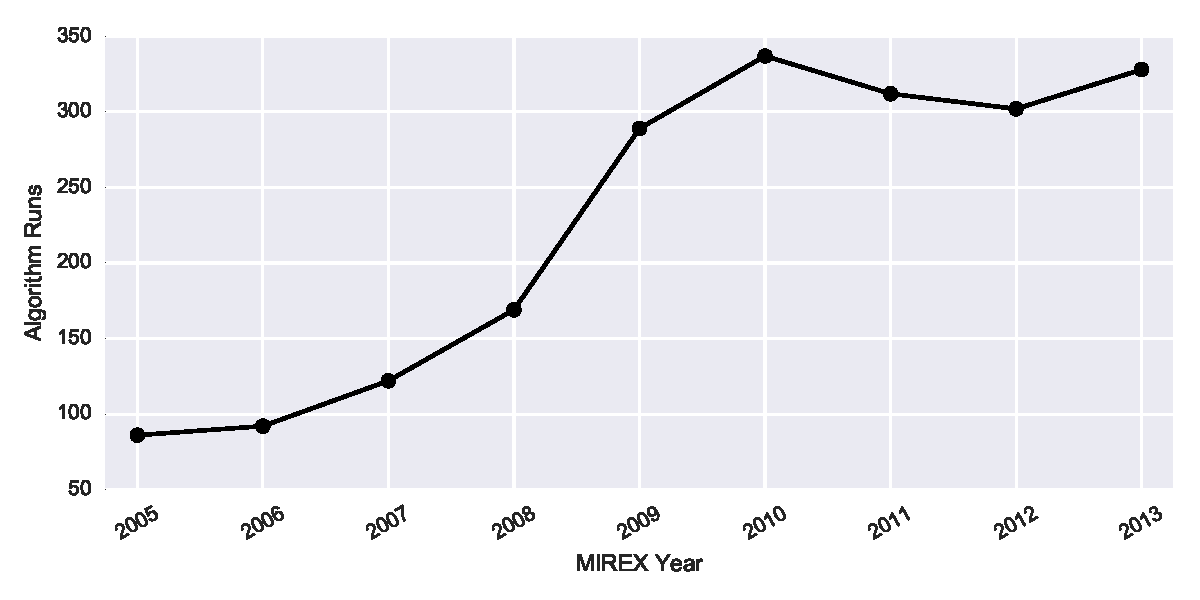
\includegraphics[width=\columnwidth]{mirex_runs}
 \caption{Number of algorithms run at MIREX over the course of almost a decade.\label{fig:mirex_participation}}
\end{figure}

% Deficiencies
% Operating costs are significant
However, experience with MIREX over the last decade has demonstrated that the decision to bring algorithms to data entails fundamental limitations.
First, as a matter of practicality, doing so incurs remarkably steep costs that the community cannot hope to sustain indefinitely.
Running hundreds of research systems demands significant computational resources, which must be either rented or purchased outright.
More often than not, these systems are research prototypes which require substantial, manual intervention to get running, and are seldom optimized for efficiency or ease-of-use.
While task-dependent runtime limits are placed on algorithm execution (between 6 and 72 hours), MIREX requires months, if not years, of annual compute-time.
% EJH: I want to mention this, but it really throws off the rhythm of this passage.
% Note that these relatively low ceilings indicate how small the datasets used in evaluation are, and more data --a universally accepted ``good thing''-- would require an increase in execution time.

The financial burden of computation can be negligible in comparison to the requisite human effort.
As a point of reference, MIREX~2007 alone required ``nearly 1000 person-hours'' to supervise the execution of 122 algorithms from 40 teams~\cite{downie2008music}.
As illustrated in \Cref{fig:mirex_participation}, the number of algorithm runs at MIREX has nearly tripled in the years since.\footnote{\url{https://www.hathitrust.org/documents/mirex_htrc_same_rda.pdf}}
%JU: One of stephen's slides (17), number of runs increases, but number of individuals decreases -> not interesting anymore
As a rough estimate, the last decade has likely consumed on the order of \emph{10,000} person-hours just bringing algorithms to data.
Not only is this rate unsustainable, but the combined operating costs only \emph{increase} with participation.
Said differently, the worst thing that could happen to MIREX in its current form is growth.


% Hard to do science
% ------------------
Operating costs aside, MIREX has indeed produced valuable insights into the development of MIR systems~\cite{downie2008music}.
Unfortunately, many scientific endeavors are largely impeded or, at worst, wholly obfuscated in the current paradigm.
To illustrate, consider the standard approach to benchmarking MIR systems as depicted in \Cref{fig:systemeval}.
An input, $X_i$, is observed by an annotator, $\mathcal{A}$, who produces a reference output, $Y_i$.
Similarly, a proposed system, $\mathcal{F}$, operates on the same input, and produces an estimate $\widehat{Y}_i$.
Each of several performance metrics, $\mathcal{M}_j$, are applied to these two representations, yielding a number of performance scores, $S_{i,j}$
This process is repeated over a sample of $n$ input-output pairs, $\{X_i, Y_i\} \in \mathcal{D}$, and the sample-wise scores are aggregated into summary statistics, $\mu$, the reliability of which generally increases with $n=|\mathcal{D}|$.

\begin{figure}
 \centering
 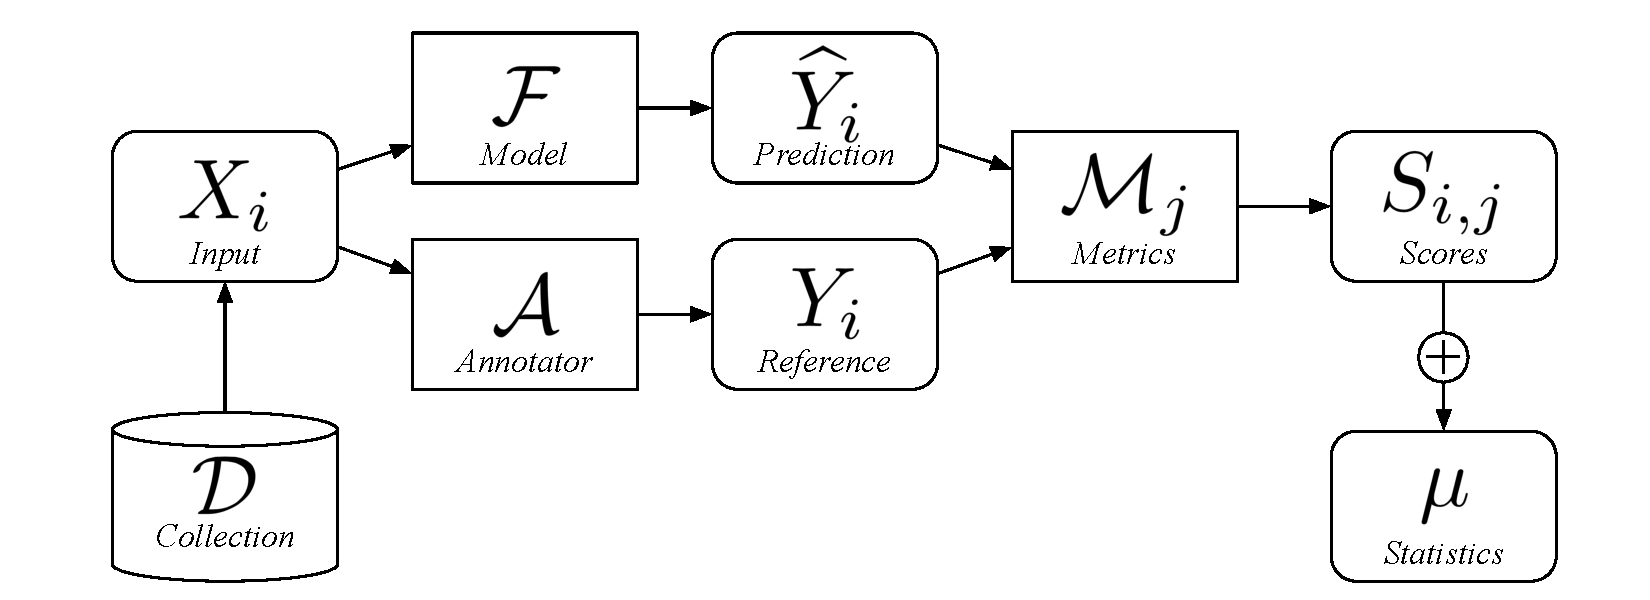
\includegraphics[width=\columnwidth]{eval_framework}
 \caption{Diagram of the standard approach to the benchmarking of MIR systems.\label{fig:systemeval}}
\end{figure}

% Transparency and oversight are necessary, this stuff is hard and warrants independent corroboration.
In the current MIREX formulation, a lack of transparency renders participants scientifically blind in a number of ways~\cite{Urbano2013:mireval}.
First, there is no intentional access to the reference annotations $Y_i$, and, in most cases, no access to the input $X_i$ as well.
Furthermore, $\widehat{Y}_i$ is largely meaningless without $X_i$ for context.
This makes it exceedingly difficult to learn from the results of the evaluation.
Without access to the underlying data, how can one diagnose the cause of an erroneous estimate, or determine ways to improve the system?
Similarly, there is no way to gauge the distribution of the data or estimate any bias in the sampling, beyond what may be inferred from public development sets or system predictions.

The behavior of the human annotators is also obscured, as are the instructions provided when the annotation was initially performed~\cite{Peeters2012:better}.
Consequently, the problem formulation itself is effectively hidden, and subject to drift over time.
For the sake of visibility into the evaluation metrics $\mathcal{M}_j$, both the original NEMA infrastructure is open source, and an ongoing community-led effort continues to standardize and improve upon these implementations~\cite{raffel2014mir_eval}.
Still, without access to the data, it is impossible to perform \emph{meta-evaluation}, or compare new metrics on old data, without seeking privileged access to the historical records.

Finally, it is only fair to admit that large scale evaluation is a considerable undertaking with plenty of room for error and misinterpretations.
Conducting these campaigns in the open makes it easier to detect and diagnose any missteps.

% Dearth Data -- MIREX is preoccupied with just keeping the ship afloat.
Somewhat ironically, due to the daunting financial and human costs of the current paradigm, the MIR community, and thus MIREX, suffers from a lack of annotated data.
This is not only detrimental to system development, but also to evaluation, because it is critical to routinely refresh the evaluation data to reduce bias and prevent statistical over-fitting.
Unsurprisingly, without a fresh source of annotated data, early concerns about the community eventually over-fitting to benchmark datasets are beginning to manifest.
In some cases, this is because the data used for evaluation exists in the wild: one submission in 2011 achieved nearly perfect scores in chord estimation due to being pre-trained on the test data.\footnote{\url{http://nema.lis.illinois.edu/nema\_out/mirex2011/results/ace/nmsd2.html}}
In other cases, participants may mis-interpret the task guidelines, as evidenced by submissions of offline systems for tasks that are online, or by others that mistakenly use annotations from previous folds in a train-test task.
Across the board, hidden evaluation data is slowly being over-fit by trial and error, as teams implicitly leverage the weak error signal across campaigns to ``improve'' systems.
These results can be misleading due to the fixed but unknown biases in the data distribution, which become apparent when datasets are expanded --- like the introduction of the Billboard dataset to the chord estimation task in 2012~\cite{burgoyne2011expert} --- or as further insight is gained, as in the disclosure of the meta-data in the music similarity corpus.

% There's no short-term plan to get new data; there's no long-term plan to get new data.
To make matters worse, there is no feasible plan in place to replenish the evaluation datasets currently used by MIREX, nor any long-term plans to replace that data when it inevitably becomes stale.
MIREX has primarily relied upon the generosity of the community to both curate and donate data for the purposes of evaluation.
This approach also struggles with transparency, making it susceptible to issues of methodology and problem formulation, and can hardly be relied upon as a regular resource.
Data collection is a challenging, unavoidable reality that demands a viable plan going forward.

After a decade of MIREX, we have learned which techniques work and which do not.
Most importantly, we have learned the importance of establishing a collective endeavor to periodically and systematically evaluate MIR systems.
Unfortunately, we have also learned of the burdens entailed by such an initiative, and the limitations of its current form.

\section{Open evaluation of MIR systems}

Summarizing the previous section, MIREX suffers from three deficiencies that render the situation untenable:
one, the financial and labor costs cannot be sustainable indefinitely;
two, the lack of data transparency limits the scientific value of the endeavor;
and three, the lack of a strategy for obtaining and annotating new data.

% Here we outline the concrete details of our proposal.
Thus, to address these deficiencies, our proposed plan has three key differentiators from the MIREX model:
\begin{itemize}
\item Distributed computation reduces operating costs to scale favorably with increased
    participation.
\item Freely distributable audio facilitates reproducibility and benefits the entire community.
\item Incremental evaluation reduces bias by keeping test data fresh, and provides a feasible strategy for collecting new data.
\end{itemize}

% After scores are released from an evaluation campaign, there is still the possibility of long-range over-fit through the feedback loop of score reporting, from which MIREX already suffers.
% To counteract this, different test collections should be introduced each year.
% At first, this seems to get us nowhere: we still need to acquire annotated data, which is presumably expensive.
%JU: I like this sentence too much to just drop it!: We argue that collecting annotations is a better use of resources (both time and funding) than maintaining server execution, as publicly available data benefits many more people than the MIREX participants for any given year.


\subsection{Distributed computation}
\label{distributed}
The primary difficulty in running an evaluation campaign is computing the outputs of all participating systems.
This difficulty stems from two sources.
First is the obvious computational complexity of running $m$ submissions over $n$ inputs.
Second is the less obvious ``human'' complexity of getting the submitted programs to execute properly in a foreign and unknown environment: a job that recently goes to the small number of task captains each year.
While the computational issues can be ameliorated by running systems in parallel over multiple machines, the cost in human effort has no easy solution in the MIREX framework.

An alternative to this framework is exemplified by Kaggle.\footnote{\url{http://kaggle.com}}
Kaggle competitions are conducted with all input data publicly available, and participants submit only the outputs of their systems, \eg, predictions made for each data point.
This paradigm effectively resolves the difficulties listed above: both computation and human effort are distributed to the participants, rather than centralized at the evaluation site and task captains.
This dramatically reduces the cost of maintenance and administration.
However, we note a few potential challenges inherent to bringing data to the computation.

First, the input data must be made openly available to participants.
This may increase the risk of bias if participants (unintentionally) tune their systems to the evaluation set.
To mitigate bias, we propose the use of a large and diverse corpus of common tracks which are shared across \emph{all tasks}, rather than a collection of small, task-specific datasets as is done in MIREX.\@
For any given task, only a subset of the data need to be considered when comparing systems, and the evaluation set may be independently selected for each task.
The knowledge of which items comprise a given evaluation subset would remain hidden from participants at submission time.
This implies that each submission must span the entire corpus, reducing the feasibility of participants tuning their algorithms to a particular subset.
Moreover, while this requirement increases computational overhead on the participant's end, it results in a large collection of outputs for various methods on a common corpus, which is a valuable data source in its own right.

Second, distributed computation entails its own challenges with respect to transparency.
While MIREX requires submissions to execute on a remote server beyond the participants' control, the scheme proposed here drops that requirement in favor of visibility into system inputs.
Consequently, restrictions on the implementation (\eg, running time) would become infeasible, and it may open the possibility of cheating by manual intervention.
Using large test collections with opaque evaluation sets will limit the practicality of
manual participant intervention.%
\footnote{Even in the unlikely event that a participant ``cheats'' by submitting human-generated annotations, the results can be publicly redistributed as free training data, so the community ultimately wins out.}
Obscuring which items belong to the evaluation subset comes at the expense of sample-wise measures, however, as doing so would reveal the partition.
This is not inherently problematic if done following the completion of a campaign, but would require changing the evaluation set annually.
These are minor concessions, and we argue that open data benefits the community at large, since its availability will serve a broader set of interests over time.

Finally, the proposed scheme assumes that multiple tasks operate on a common input form, \ie, recorded audio.
While the majority of current MIREX tasks do fit into this framework, at present it precludes which require additional input data (score following, singing voice separation) or user interaction (grand challenges, query-by-humming/tapping).
Our long-term plan is to devise ways of incorporating these tasks as well, while keeping with the principles outlined above.
This is of course an open question for further research.


\subsection{Open content}
\label{open}

For the distributed computation model to be practical, we first need a source of diverse, representative, and freely distributable audio content.
Free audio content is significantly easier to acquire now than when MIREX began in 2005, and in particular, a wealth of data can be obtained from Jamendo~\footnote{\url{http://jamendo.com}} and the Free Music Archive (FMA).\footnote{\url{http://freemusicarchive.org/}}
Both of these sites host a variety of music content under either public domain or Creative Commons (CC) licenses.\footnote{\url{https://creativecommons.org/licenses/}}
Since CC-licensed music can be freely redistributed (with attribution), it is (legally) possible to create and share persistent data archives.

The Jamendo and FMA collections are both large and diverse, and both can be linked to meta-data: Jamendo via DBTune to MusicBrainz~\cite{raimond2008web} and FMA to Echo Nest identifiers.
Jamendo claims over 500,000 tracks charted under six major categories: \emph{classical}, \emph{electronic}, \emph{hip-hop}, \emph{jazz}, \emph{pop}, and \emph{rock}.
FMA houses approximately 90,000 tracks which are charted under fifteen categories: \emph{blues}, \emph{classical}, \emph{country}, \emph{electronic}, \emph{experimental}, \emph{folk}, \emph{hip-hop}, \emph{instrumental}, \emph{international}, \emph{jazz}, \emph{old-time/historic}, \emph{pop}, \emph{rock}, \emph{soul/rnb}, and \emph{spoken}.
These categories should not necessarily be taken as ground truth annotations, but they reflect the tastes and priorities of their respective user communities.
While there is undoubtedly a strong western bias in these corpora, the same is (almost certainly) the case in MIREX's private data and the MIR field itself, but using open content at least permits practitioners to quantify it.

This now leads us to the question of representation.
A common criticism of basing research on CC-licensed music is that the music is of substantially lower ``quality'' --- which may refer to either artistry or production value, or both --- than commercial music.
This point is obviously valid for high-level tasks such as recommendation, which depend on a variety of cultural, semantic, and subjective factors beyond the raw acoustic content of a track.
However, for the majority of MIREX tasks, in particular the low-level tasks such as beat-tracking or key estimation, this is a much more tenuous case.
We note that FMA includes content by a variety of commercially successful artists,\footnote{\url{https://en.wikipedia.org/wiki/Free_Music_Archive#Notable_artists}} but the vast majority of content in both sources is provided by relatively unknown artists, which makes it difficult to control for ``quality''.

To help users navigate the collections, both Jamendo and FMA provide popularity-based charts and community-based curation, in addition to the previously mentioned genre categories.
Taken in combination, these features can be leveraged to pre-emptively filter the collections down to subsets of tracks which are either of interest to a large number of listeners, of interest to a small number of listeners with specific tastes, or representative of particular styles.
This approach is similar in spirit to previous work using chart-based sampling (typically Billboard)~\cite{burgoyne2011expert}.

% provide a snapshot torrent for each year's data set
% including for each track:
%   audio
%   metadata (via musicbrainz ids)
%   cc attribution

% what can we say about quality control?
%   maybe do something similar to how MSD was constructed
%       1/3 popular stuff (by play count)
%       1/3 uniform sampling by genre
%       1/3 some random dregs
%   each year, add a sampling of tracks added within the last year

% QC can also happen in evaluation set selection
%   look for disagreements per method
%   when soliciting annotations, allow annotators to flag tracks which are bad for the
%   given task (under an appropriate definition of ``bad'')
%   also solicit confidence ratings in the annotations

\subsection{Incremental evaluation}

In its first cycle of operation, the proposed framework requires a new, unannotated corpus of audio.
Rather than fully annotate the corpus up front for each task, we plan to adopt an \emph{incremental evaluation} strategy.

With incremental evaluation, the set of reference annotations need not be complete: some (most) input examples will not have corresponding annotations.
% BM: do we have a reference for incremental evaluation?
%The idea is to develop methods to estimate these missing annotations from all available sources of information, such as existing annotations, metadata, system outputs, \etc.
%Annotations will therefore be defined probabilistically, over the space of possible labels, so that missing annotations will have some degree of variance (uncertainty); existing annotations will have zero-variance.
Instead, performance measures are estimated with respect to a subset of annotated tracks, which may itself grow over time.
%With an appropriate reformulation of performance measures, we can incorporate these estimates of the annotations and produce estimates of the system performance scores.
Systems are ranked as usual, but with some degree of uncertainty which is inversely proportional to the number of available annotations.

Initially, uncertainty in the performance estimates will be maximal, due to a small number of available annotations.
Subsequently, as reference annotations are collected and integrated to the evaluation system, they will be compared to the submissions' estimated annotations, providing incrementally better estimates of each system's performance.
Prior research in both text and video IR has demonstrated that evaluation against incomplete reference data is feasible, even when only a small fraction of the annotations are known~\cite{Carterette2007:robust,Yilmaz2008:simple,trecvid2014:overview}.

One point to study in this framework is: which inputs are worth annotating?
Consider two systems that produce the same annotation for a fixed input example.
Whether they are both right or wrong with respect to a reference, there is no way to distinguish between them according to that example, so there is little value in seeking its annotation.
Conversely, examples upon which multiple systems \emph{disagree} are more likely to produce useful information for distinguishing among competing systems.
%Annotating every track for every task would be a monumental undertaking, and an inefficient use of resources.
Several recent studies have investigated the use of algorithm disagreement for this issue, be it for beat tracking~\cite{holzapfel2012selective}, structural analysis~\cite[chapter 4]{nieto2015discovering}, or chord recognition~\cite{humphrey2015fourtimely}.
Others have studied alternative methods for music similarity~\cite{Urbano2013:mtc}, choosing for annotation the examples that will be most informative for differentiating between systems.
In general, these methods allow us to minimize the required annotator effort by prioritizing the most informative examples.
With many participating systems, and multiple complex performance metrics, prioritizing data for annotation is by no means an obvious task.
We hope that the community will assist in specifying these procedures for each task.

In the proposed framework, annotations may come from different sources, so it is imperative that we can trust or validate whatever information is submitted as reference data.
Another line of work is thus the development and enforcement of standards, guidelines and tools to collect and manage annotations.
This will probably involve the development of both desktop and web technologies for creating and managing annotations, as well as appropriate versioning and quality control mechanisms.
Quality control is particularly important if annotations are collected via crowd-sourcing platforms like Amazon Mechanical Turk.\footnote{\url{https://www.mturk.com/}}
%The intuition for this approach is two-fold.
%First, tracks for which different algorithms produce significantly different outputs are in some sense ``difficult'' and produce meaningful evaluation results.
%Second, if a goal of the evaluation campaign is to differentiate submissions according to some measure of accuracy, then there is little to be gained by spending annotator effort on tracks for which algorithms produce the same output.

%In the proposed framework, we are in a fortunate position of having exactly this type of functionality available to us: participants are submitting system outputs for evaluation!
%It need not be the case that all of the data is being used for evaluation: in fact, Kaggle shows that it is helpful to cloud the space with data that are not included in testing.
%If we are careful about selecting these data, we can then compare the outputs across the participating systems to see which ones are ``interesting'': if the systems generally agree, the example is likely to be easy; at the very least, annotating this track will not help distinguish between these systems.
%If the systems disagree, then we should definitely solicit a strong annotation for the track.
%This is essentially the point made by Urbano et al. %\cite{2012UrbanoXYZ}.

%Each track marked as ``interesting'' should be annotated by at least two humans to determine whether there is actual disagreement.
%It can then be annotated in year 2, and enter the evaluation in year 3.
%By having multiple reference annotations for the ``interesting'' tracks, we can compare algorithm agreement to annotator agreement, and distinguish ``difficult'' tracks from ``ambiguous'' tracks.

%Finally, the fourth point above can be integrated into point 2 by soliciting recommendations from the community.

%Additionally:
%\begin{itemize}
%\item Annotation Standards and their enforcement
%\item User-facing tools for performing annotations
%\item Backend infrastructure for hosting, serving, and collecting submitted annotations (common repository)
%\item Would it be possible to leverage citizen science platforms, Mechanical Turk, etc
%\end{itemize}

\subsection{Putting it all together}

In contrast to the outline in \Cref{sec:mirex}, our proposed strategy could proceed as follows:
\begin{enumerate}
\item Identify and collect CC-licensed audio data.
\item Define or update tasks, \eg, chord transcription.
\item Release a collection of (annotated) training data for development, and an over-complete collection of unlabeled data for evaluation.
\item Invite participants to submit \emph{predictions} over the unlabeled data.
\item Collect reference annotations; prioritize examples by disagreement among submissions.
\item Estimate and summarize each submission's performance against the reference annotations.
\item Retire annotated data, and add it to the training set for the next campaign.
\item Go to step 3 and repeat. Revisit steps 1--2 if needed.
\end{enumerate}


Steps 1--3 essentially constitute the startup cost, and are unavoidable for tasks which lack existing, open data sets.
However, from the perspective of administration, only steps 3 and 5 require significant human intervention (\ie, annotation), and both steps directly result in public goods.
In this way, the proposed system will be significantly more efficient and cost-effective than MIREX.\@

% TODO: Much of this can be consolidated, serving to support the enumerated list above, rather than conveying it. There's still some good bits here, so leaving for now. Important bits to touch on include
%  * Spooling data collection
%  * Any fund-raising efforts can be allocated to data collection, rather than operating costs. We've had success raising money, but we could be using those funds differently.
% ---
% First is the \emph{Content Selection} stage.
% Here, we provide ``stale'' annotated data --that which shouldn't be used for evaluation any longer-- as training data.
% Then, to curate a test set, we combine data previously unseen by the community for which we have annotations, with new, unlabeled content.
% This unlabeled content serves to both obscure the data-points in the test set that \emph{are} annotated, as well as solicit predictions from a large number of automatic algorithms.

% Next is the \emph{Competition}, a time-boxed interval spanning a few weeks or months.
% Content is made available publicly available is made at the start, such that the training set is provided with labels and the entire test set, without. Some number of submissions are accepted over this internal from registered participants.
% A standard format for predictions is defined for each task, and participants can check their submissions against a evaluator to immediately an inkling of how they perform.
% This public leader-board gives insight on some percent of the data. e.g. Kaggle, and at the end of the competition, results are tabulated over the entire holdout set.

% After the completion officially closes comes \emph{Incremental Evaluation}. Using the predictions submitted, identify content worth annotating.
% It is at this point we can additionally revisit questionable annotations, and perform meta-evalatuation of our common methodology.

% Having identified content worthy of investing human effort, the \emph{Annotation} stage proceeds until the next competition.
% This is an important distinction, as it takes the most time consuming process --humans describing music-- and largely decouples it as an independent resources.
% Thus, annotation spools constantly as a background process, and a snapshot

% This virtuous cycle can then repeat indefinitely.
% Some particularities are worth mentioning.
% For example, it may be necessary to include humans in the evaluation loop at the close of the competition stage, as in user-facing challenges or music similarity ranking.


\section{Discussion}

%What follows are a number of topics that have cropped up in the course of writing the paper to date.
In this section, we elaborate on a number of facets related to the overall goals and actualization of the proposed framework.

\subsection{Why now?}

The challenges described in this document, which our proposed strategy aims to address, are not news to the community.
The operating costs of MIREX became apparent early in its lifetime, and concerns about its sustainability loom large among researchers.
In parallel, data collection is inherently difficult;
if it were easy, there would be less motivation to develop automatic annotation systems.
This begs an obvious question: why \emph{now}?

% We're in a different day and age.
The answer, of course, is that timing is everything.
In many ways, the approach taken by MIREX made perfect sense in the early 2000's.
%However, the modern era provides a far more hospitable environment than the one for which it was designed.
However, recent infrastructural advances, coupled with growth and maturation of the MIR community, have introduced new possibilities.

% The open source audio content game has changed dramatically, we can now build datasets around open content.
First and foremost, creative commons music is now ample, bringing the dream of sharing data within grasp.
% Operating costs are minimal.
Cloud computing is cheap and ubiquitous, which can dramatically reduce the administrative costs of evaluation infrastructure and persistent data storage.
Improvements in web infrastructure have made the distribution of large-scale data sets to participants is now feasible.
% Tools and technologies are better, JavaScript support, HTML5, python, etc.
Similarly, browser support for interactive applications enables the development of web-based annotation tools, which significantly reduces the barrier to entry for annotators.

% We're ready for it.
Finally, the community has matured significantly since MIREX began in 2005.
Open source development and reproducible methods are now commonplace, but we remain hindered by the lack of open data for evaluation.
Only by developing frameworks for open evaluation and data collection, can we further develop as a scientific discipline.


\subsection{Implementation details}
\label{sec:implementation}
% Hosting datasets, torrents + edu labs.
% We'll need some infrastructure to actually run the campaign in the new setup.
% I think CodaLab might have solved a good chunk of this problem for us.
% Evaluation machinery, mir\_eval.
Effectively deploying the proposed framework will require two things: infrastructure development, and hosting.
On the infrastructure side, we can leverage several existing open source projects: \texttt{mir\_eval} for scoring~\cite{raffel2014mir_eval}, JAMS for data format standardization~\cite{humphrey2014jams}, and CodaLab for running the evaluation campaign.\footnote{\url{http://codalab.org/}}
The last remaining software component is a platform for collecting annotations.
% Web tools, front-end dev work.
In addition to traditional desktop software, browser-supported annotation tools would facilitate data collection immensely, and a content management system could field annotations as they are completed.
% Fortunately, as mentioned above, the tools and technologies available to achieve these goals have only gotten better in the last decade.

As for hosting, since the burden of executing arbitrary (submitted) code is removed, the remaining software components can reside on either a private university server, or, more likely, cloud-based hosting such as Amazon Web Services.\footnote{\url{https://aws.amazon.com/}}
Similarly, the audio data can be distributed via BitTorrent to participants, or hosted (at some minor cost) for traditional download.

%We may also consider a two-tiered system, in which closed systems are ranked separately from open systems, which provide voluntary source code.
%This may help ease the burden of going fully open source, and encourage submissions from industry.
%I think this is a bad idea though.
%If it isn't open, it isn't science.
%(Just make it cost money then. Which would require the org to NPO-ize).


\subsection{Data and evaluation Integrity}

% Participant Honesty -- we've already harped on this twice now, so we should chose our words carefully (or succintly)
Allowing participants to submit predictions, rather than software, may raise questions about integrity:
how can we verify the process which generated the predictions?
Ultimately, we must rely on participants to be honest in describing their methods.
Although it is \emph{possible} for a participant to manually annotate each track and achieve high scores, we hope that the scale of the dataset will make this approach fundamentally impractical.
Additionally, in keeping with the spirit of open science and reproducible methods, we will encourage participants to link to a repository containing their software implementation, which can be used to independently verify the predictions.

% System integrity
%We may also encourage (require?) participants to release source code to reproduce their methods.
%This is in keeping with the spirit of open science and reproducible methods.
%I doubt there will be any way to enforce this systematically, but it could be used to audit systems post-hoc.
%Kaggle requires prize winners to open source their systems.

% Data integrity
% Data integrity, creative commons content.
When it comes to data integrity, we acknowledge that music is unique in that its perception is impacted by a plethora of cultural and experiential factors.
In particular, CC-licensed music may lie outside of the gamut of commonly studied music, and differences in compositional style, instrumentation, or production, may lead to difficulties in validation and generalization.
While this is unlikely to impact low-level tasks such as onset detection or instrument identification, more abstract tasks, such as chord estimation or structural analysis, may be more sensitive to selection bias.
Relying on curation and chart popularity as a pre-filter in data selection may help to mitigate these effects.
After collecting an initial set of annotated CC-licensed music, it will be possible to quantitatively measure the differences in system performance compared to existing corpora of commercial music.


\subsection{Collecting annotations}

Statistically valid evaluation requires a continuous source of freshly annotated data.
Here, we identify three potential annotation sources.

% Get funding and pay for it.
First is the traditional route of raising funds and paying expert annotators.
This option incurs both a direct financial cost and various hidden human costs, but is also the most likely to produce high-quality data, and may in fact be the only viable path for certain tasks.
In the grand scheme of things, however, the financial burden may not be so severe.
As a point of reference, MedleyDB, a well-curated dataset of over 100 multi-track recordings for a number of MIR tasks, cost approximately \$12 per track to annotate (\$1240 total)~\cite{bittner2014medleydb}.\footnote{Figures provided via personal communication with the authors.}
The ISMIR Society maintains a membership of roughly 250 individuals each year:
a \$5 increase in membership dues would cover the annotation cost of a new dataset like MedleyDB annually.
Grants or partnerships with industry could also offset the cost of annotation.

% Crowd-sourced
Second, for tasks that require minimal annotator training, we can leverage either crowd-sourcing platforms, \eg, Mechanical Turk, or seek out enthusiastic communities interested in voluntary \emph{citizen science} for music.
Websites such as Genius\footnote{\url{http://genius.com/}} (6M monthly active users) and
Ultimate~Guitar\footnote{\url{http://www.ultimate-guitar.com/}} (3M monthly active users) demonstrate the existence of these communities for lyrics and guitar tablature.\footnote{Data gathered from \url{http://compete.com}, March 2016}
% Clear need and interest, hook into the community.
As witnessed by the success of eBird\footnote{\url{http://ebird.org/}} or AcousticBrainz,\footnote{\url{http://acousticbrainz.org/}} great things happen when you empower crowds of intrinsically motivated people.
% If we build it, they will almost certainly come; in some cases, they're already there.

% Self-supported
Finally, if no funding can be found to annotate data, we may solicit annotations directly from participants and the ISMIR community at large.

In each case, we will institute a ratification system so that annotations are validated by a third party before being accepted into the evaluation set.
As mentioned in \cref{sec:implementation}, web-based annotation tools will enable volunteer contribution, in addition to any paid annotator.


%To participate in an evaluation, each participant must ``pay''� some nominal amount of data credits.
%In the first year, all participants start with a balance of 0, so by participating, they are now in ``data debt''�.
%Data credits can be earned by providing annotations to be used in the following year's campaign.
%A participant is eligible for evaluation in year $X$ when their data credit reaches a non-negative value.
%
%Data credits can be retained across years, and transferred across tasks.

%The credits earned can be task-dependent.  Chord annotations might be worth more than beat timings or tempo estimations, for instance.

%Data credits may also be earned at a discounted rate by auditing or validating previously provided annotations?  We'll need a system in place to authenticate annotators and force independence.

%Potentially, we may institute a cap-and-trade system to exchange data credits for money which can be used to pay for expert annotations.  Not sure about the legal ramifications of implementing this, or how to organize efforts.  Aside from cash exchange, there might be a benefit to having a task exchange: eg, ``ill trade three beat annotations for one chord annotation�.


\section{Next steps: A trial run}

% How do we get people to participate / contribute (all jump at once).

We conclude this proposal by advocating a large-scale instrument identification task for ISMIR2017.
% What is the task?
In this task, the presence of active instruments (under a pre-defined taxonomy) are estimated over an entire recording.
The taxonomy may be readily adapted from WordNet~\cite{miller1995wordnet}, and refined by the community, starting at this year's ISMIR conference.
% Motivations
There are a number of strong motivations for pursuing instrument identification.
% Good MIR problem, let's finally solve something.
It is an important, classic problem in MIR, but one currently missing from MIREX.\@
Researchers typically explore the topic with disparate, often unrealistic datasets, and the problem remains unsolved to some unknown degree.
% Relatively easy / stable data collection
Compared with other music perception tasks, annotation requires a simple interface, \eg, ``check all that
apply'', and the task definition itself is relatively objective: a particular instrument is either present in the mix or not.%
%\footnote{Granted, synthesizers wreak havoc on any taxonomy; computer vision faces similar issues with natural images of paintings, for example.}
% Content validity.
Instrument occurrence is largely independent of popularity, which results in a fairly minimal bias due to the
use of CC-licensed music.
% Epic win for the community.
Finally, computer vision found fantastic success with a parallel endeavor, known as ImageNet~\cite{deng2009imagenet}, in which algorithms detect objects in natural images.
%ImageNet has proven to be an invaluable resource, not only advancing research to solve that particular task, but also sparking other investigations, such as Google's now-famous Deep Dream\cite{}.
% This offers the benefit of draw other researchers into MIR, and in some ways legitimize the field.

There are several prerequisite steps to realize this goal within the coming year.
One, we must establish a robust instrument taxonomy as a community, a key to ImageNet's success;
two, acquire a large sample of audio content;
three, build a web-based annotation tool and storage system;
four, consolidate existing datasets into a common format as a development set;
five, implement or collect a few simple algorithms to prioritize content for initial annotation;
six, perform data collection, through some combination of paid annotation, crowd-sourcing, and community support;
and finally, deploy an evaluation server and leader-board to accept and score submissions.
Each of these components, while requiring some engineering and organization effort, are certainly achievable goals with the help of the ISMIR community.


% \section{Misc Refs}
% Separate ``labels�'' for systems depending on what they do (eg. close/open, full/subset of dataset): http://trec.nist.gov/pubs/trec22/papers/WEB.OVERVIEW.pdf
% Previous proposals (section 8): http://julian-urbano.info/files/publications/051-evaluation-music-information-retrieval.pdf


% For bibtex users:
\bibliography{ISMIRtemplate}

\end{document}

